\chapter{The Level-1 Trigger upgrade jet algorithm}
\label{chap:l1trig}

\section{The Calorimeter Trigger upgrade for Run~2}
\label{sec:trigUpgrade}

With the advent of Run~2 of the \LHC, the demands placed on the \CMS
trigger greatly increased. After a long period of shutdown the energy
of proton collisions was increased to $13~\tev$ and the bunch crossing
rate decreased to 25~ns. With this configuration the design luminosity
of $10^{34}$cm$^{-2}$s$^{-1}$ can be reached with an average \PU of
around 25 events per bunch crossing. However, the potential luminosity
of the \LHC after the pre-Run~2 upgrade exceeds the original design
value, allowing a \PU of up to 40. As the original Level-1 trigger was
not designed to deal with this degree of \PU, its performance would be
significantly diminished. The presence of extra collisions in each
event results in a general increase in the average energy deposited in
the calorimeters of the detector. This extra energy smears out the
measurement of energy deposited from the primary vertex, reducing the resolution with
which it is measured. This acts to increase the rate at which the
trigger accepts events and decrease the accuracy with which it
identifies interesting events. As this rate is limited by the readout
capability, a trigger that is not upgraded will have a reduced
efficiency of acceptance of interesting physics events.  It is
therefore very advantageous to upgrade the Level-1 trigger in a way
that allows it to deal with the extra \PU \cite{Tapper:1556311}.

Along with maintaining a low output rate and a high efficiency,
another key consideration for the Level-1 trigger is the latency of
the algorithms run on the boards that carry out the trigger
processing. The latency must be kept low to ensure that each bunch
crossing can be processed in as much detail as possible. To be able to
carry out this sort of processing the Level-1 makes use of custom
\FPGA boards, as described in . The complexity and structure of the
trigger algorithms is therefore limited to ensure they can run quickly
enough on the \FPGA boards. An upgrade to the trigger hardware
therefore allows more sophisticated algorithms to be carried out,
while still being able to process every bunch crossing.

The amount of calorimeter information that can be put into a single
\FPGA is also limited by its I/O capacity. To process the full
calorimeter data from a single bunch crossing in the Level-1 trigger
it takes the equivalent of $\sim10$ bunch crossings of time. In Run~1
of the \LHC the calculations for triggering on the calorimeters were
performed with the \ac{GCT}.The \ac{GCT} dealt with this delay by
processing different sections of the calorimeter in separate boards,
necessitating duplication of information at the detector section
boundaries. However, by time multiplexing the calorimeter data, it is
possible to have individual \FPGA boards that each process one bunch
crossing with minimal information duplication. As well increasing the
possible information bandwidth, this allows much greater flexibility
in algorithms as each \FPGA has access to all the information available
in each event \cite{1748-0221-9-10-C10034,1748-0221-7-01-C01060}. 

\begin{figure}[!t]
  \centering
  \subfloat[Run~1 trigger architecture.]{
    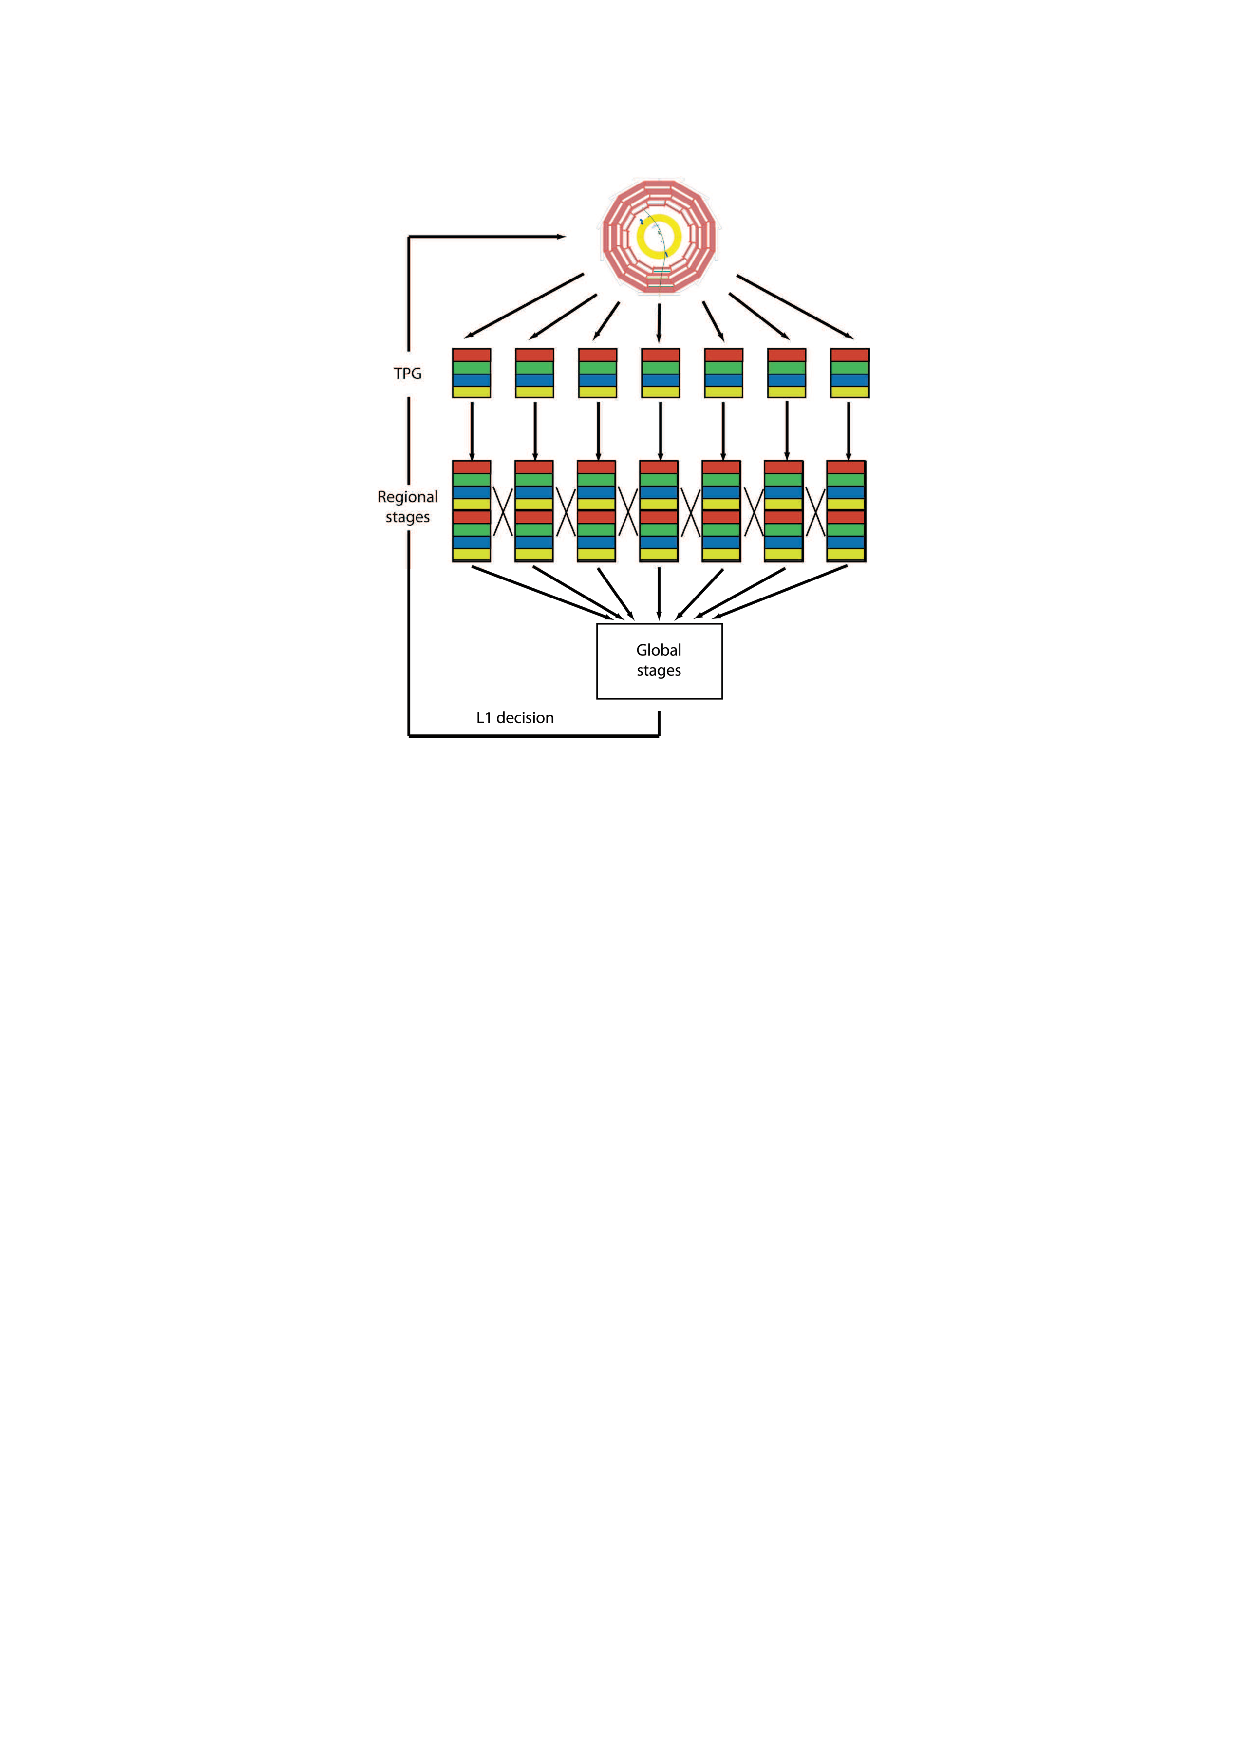
\includegraphics[width=0.4\textwidth]{figs/trigger/old_trigger}
  }~~
  \subfloat[Run~2 upgrade TMT trigger architecture.]{
    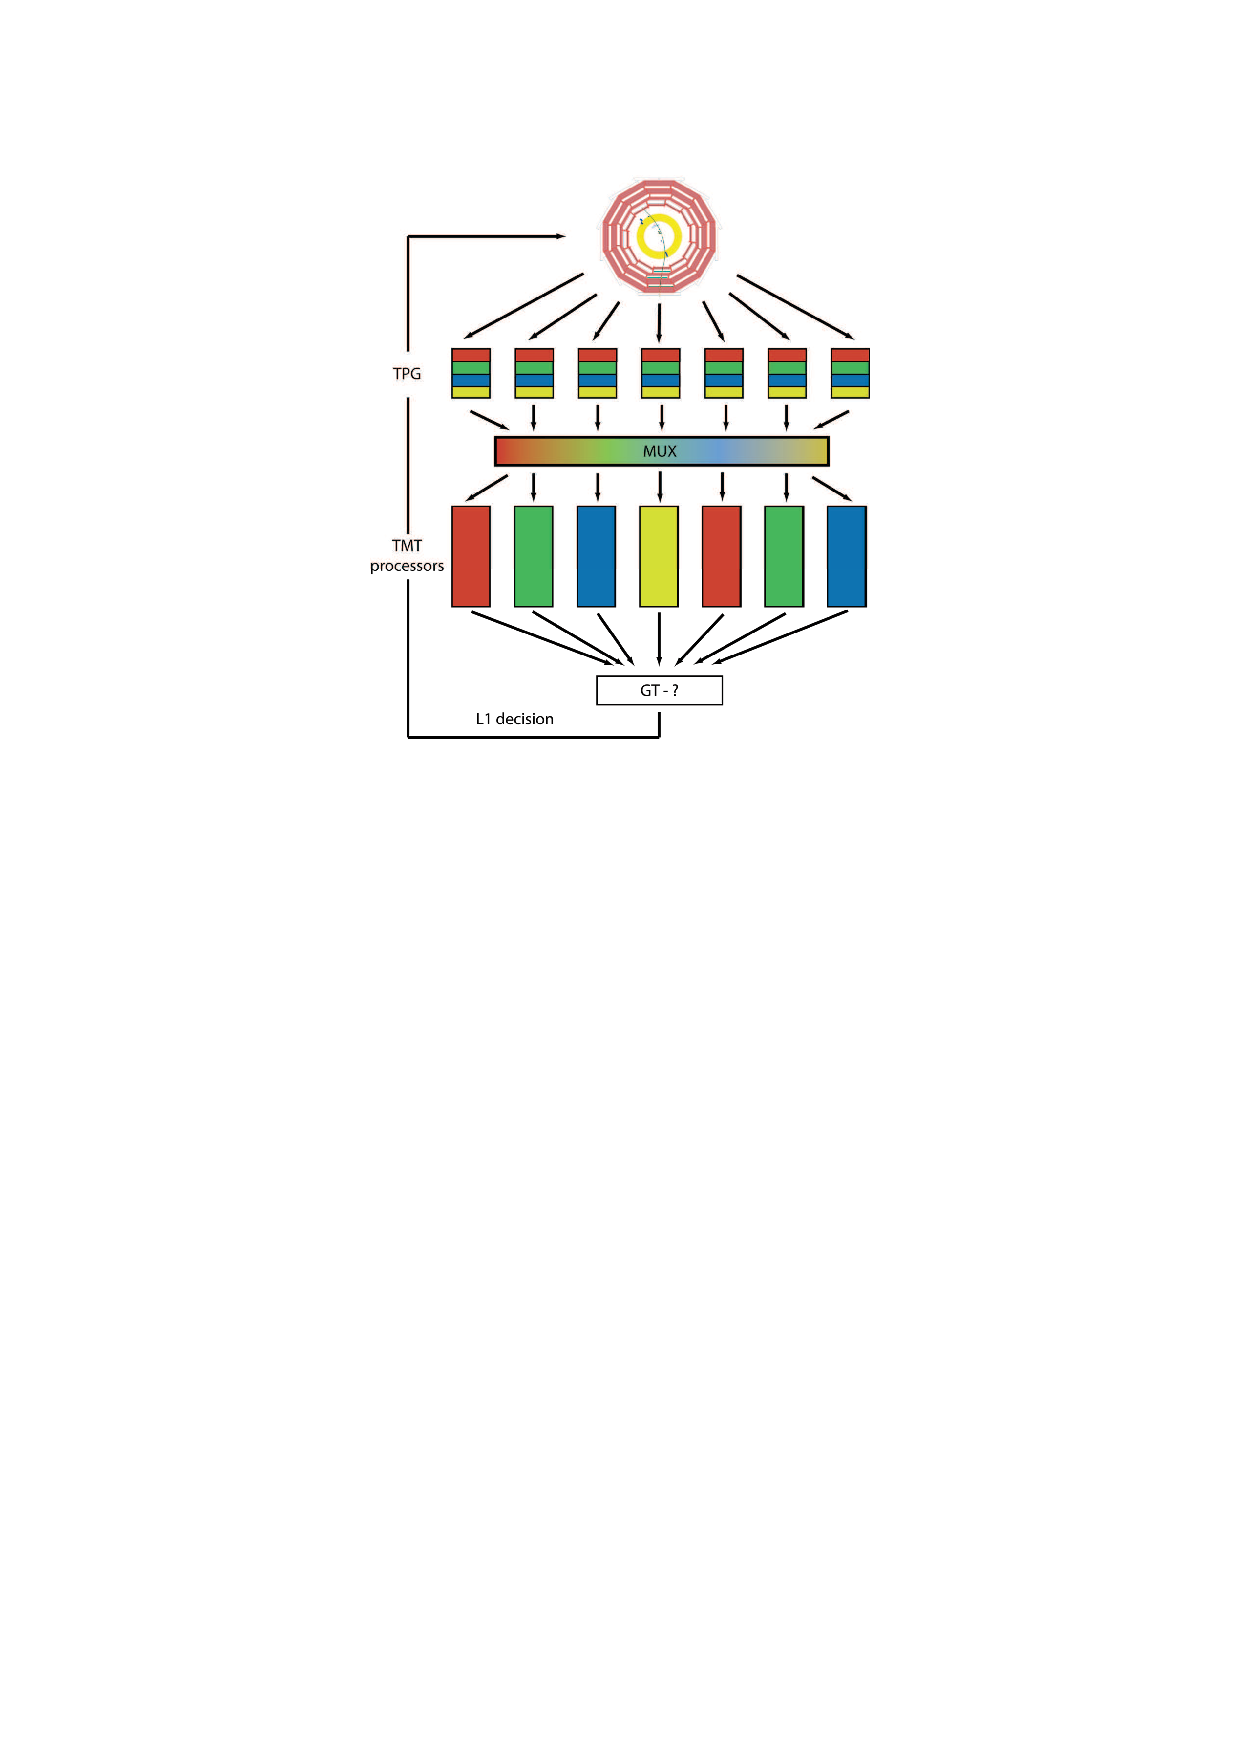
\includegraphics[width=0.4\textwidth]{figs/trigger/tmt}
  } \\
  \caption{A representation of the time multiplexed trigger (TMT)
  architecture (b) as opposed to the pre-upgrade trigger architecture
  (a). The entire information for one event is processed by one board
  rather than just parts of the detector for each board \cite{1748-0221-9-10-C10034}}
  \label{fig:tmt}
\end{figure}

The upgrade to the Level-1 trigger exploits the recent technological
improvement in the performance of \FPGA processors and high-speed
optical linksi \cite{tp}. The upgrade architecture is that of a \TMT, a 
representation of the difference between this architecture and that of
the \ac{GCT} can be seen in Fig.~\ref{fig:tmt}.

The inputs to the Calorimeter Trigger from the varous \ECAL and \HCAL
components are split into a $56\times 72$ grid of \TT in $\eta$ and
$\phi$, with each tower covering the area of $5\times5$ \ECAL crystals.
As the processing power of the \ac{GCT} was limited, for trigger
calculations the \TT were grouped into $4\times4$ blocks, known as
\emph{RCT regions}. These different regions are visually represented
in Fig.~\ref{fig:trigger_calorimeter}. Due to the advantages brought
by the upgrade, the new algorithms will have access to the full
granularity information of all the \TT. A representation of the
upgrade to the position resolution presented by this change is in
Fig.~\ref{fig:sunnyJim}.

\begin{figure}
	\begin{center}
		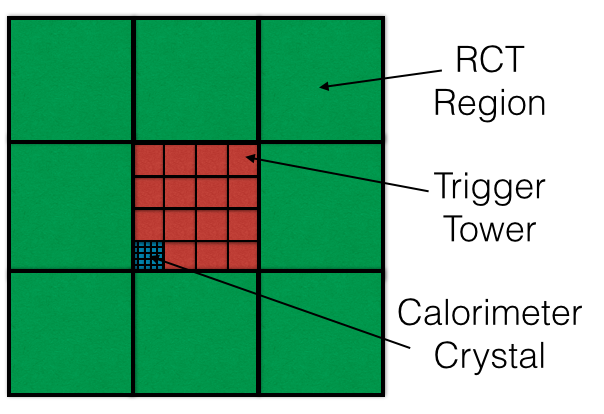
\includegraphics[width=0.7\linewidth]{figs/trigger/trigger_calorimeter}
	\end{center}
	\caption{The breakdown of the different calorimeter regions, the RCT
  and trigger towers are both }
	\label{fig:trigger_calorimeter}
\end{figure}

\begin{figure}[!t]
  \centering
  \subfloat[Run~1 calorimeter trigger resolution.]{
    
\includegraphics[width=0.5\textwidth]{figs/trigger/L1inputreslegacy}
  }~ 
  \subfloat[Run~2 upgrade trigger resolution.]{
    
\includegraphics[width=0.5\textwidth]{figs/trigger/L1inputresupgrade}
  } \\
  \caption{A representation of the position resolution of the trigger
  inputs to the calorimeter trigger for the Level-1 trigger before and
  after the upgrade.}
  \label{fig:sunnyJim}
\end{figure}


\section{The jet finder and energy sums}
\label{sec:jetFinder}

To make use of the potential brought by the Level-1 trigger upgrade,
new trigger algorithms improve the identification of different physics
processes. With higher granularity information available, it is
possible to develop triggers with a significant performance upgrade
when identifying the objects required in the various analyses carried
out as part of the \CMS physics programme.  With a better view of the
substructure of energy deposits within the calorimeters the
identification of three pronged tau jets and isolated electrons can be
significantly improved, for example \cite{egllr,taullr}. 

One particular area for improvement is in the jet algorithm.  As the
Level-1 trigger must be of a fixed latency it cannot make use of an
iterative algorithm, such as those used during offline jet-finding
(described in Sec.~\ref{sec:jets_reco}).  During Run~1, the jet
candidates were created from a $3\times3$ RCT region sliding window.
Candidates in which the central region has the maximum energy are kept
as jets. These jets cover an area of $\Delta\eta\times\Delta\phi =
1.04 \times 1.04$, which matches reasonably well the $R=0.5$ maximum
radius for Run~1 offline jets. To help mitigate the reconstruction of jets
originating from \PU the central region of the jet finder is also
required to exceed a minimum energy, known as the \emph{seed
threshold}. However, the contribution to the energy of the jet from
\PU cannot be subtracted dynamically. Along with the relatively large jet size the
performance of this algorithm will therefore be severely reduced by the
conditions that will be experienced during Run~2. The upgrade will
provide the extra processing power aim to carry out a dynamic \PUS,
correcting the energy present in each jet. The increased position
resolution will also allow for a more accurate determination of the
direction of the jets

\subsection{The upgraded jet algorithm}
\label{sec:stage2_jetalgo}

The jet algorithm for Stage 2 of the CMS trigger upgrade operates on
the sum of the \ECAL and \HCAL energy deposits in the \TT. The studies
in this Chapter consider the \TT within $|\eta|<3$, with the potential
to extend the algorithm up to $|\eta|<5$. 

Starting with a similar idea as in Run~1, the upgrade makes use of a
sliding window algorithm. In the upgrade, however, the window
considered is a $9\times9$ square of \TT, covering
$\Delta\eta\times\Delta\phi = 0.78 \times 0.78$. This odd number of
trigger towers results in an easily defined local maximum as well as
matching the $R=0.4$ Run~2 radius of offline jets. Within a window the
central tower is considered as the direction of a candidate jet. The
candidate is vetoed if any of the other \TT in the square have an
energy deposit of either greater than or greater than or equal to it.
The veto condition applied is antisymmetric along the diagonal of the
square to prevent \TT with the same energy from vetoing one another. A
representation of this window considered can be seen in
Fig.~\ref{fig:stage2_jetalgo}.  Any \TT that pass this criteria are
considered as jet centres, where the jet energy is equal to the sum of
all the towers within the $9\times9$ square.
% Taking the highest energy
% TT as the centre of the jet axis is motivated by the fact that jets
% are boosted objects with most of their energy in the middle
% \cite{JetProfile_pileup}.

The veto conditions applied on the central TT ensure that no two
overlapping jets are reconstructed, avoiding the duplication of energy
deposits. However, the algorithm can introduce inefficiencies in very
specific jet topologies. In these cases a high energy TT vetoes a
medium energy TT which then vetoes a lower energy TT. In this case the
medium TT is included in the jet constructed by the high energy TT,
however the lower energy TT is lost. This is not usually a problem
from the Level-1 Trigger point of view, as the high energy TT will
usually ensure that the event is triggered, despite energy being lost.

\begin{figure}
	\begin{center}
		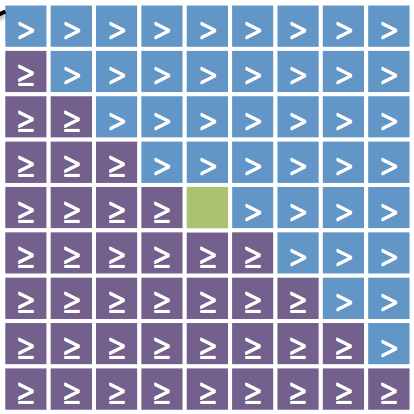
\includegraphics[width=0.4\linewidth]{figs/trigger/stage2_jetalgo}
  \end{center} \caption{The consideration of a Trigger Tower candidate
  for the upgrade Level-1 Trigger jet algorithm. The candidate (green)
  is vetoed if the energy of the other towers meets the condition
  shown in the blue and purple towers.}
	\label{fig:stage2_jetalgo}
\end{figure}

\subsection{A comparison with the offline jet algorithm}

In order to test the performance of the algorithm it is compared to
jet finding with anti-$k_T$ clustering, the most popular algorithm
used for offline jet reconstruction. As the Level-1 algorithm has less
sophisticated inputs than the \PF candidates used offline, the
anti-$k_T$ algorithm is used to find jets with the \TT. The test was
carried out on a top pair-production \MC sample, due to the high
multiplicity of jets produced in top-quark decays. The performance of
the algorithm compared to offline jet reconstruction with $R=0.4$ can
be seen in Fig.~\ref{fig:ak4_comp}. For the jet with the highest \pT,
the leading jet, the distributions of \pT and $\eta$ are very similar
for both the jet finding algorithms. For the fourth-leading jet more
differences emerge at low \pT and the edges of the $\eta$
distribution. This is probably due to the ability of the anti-$k_T$
algorithm to adaptively fit smaller radius jets and those at the edge
of the detector acceptance.

\begin{figure}
	\begin{center}
		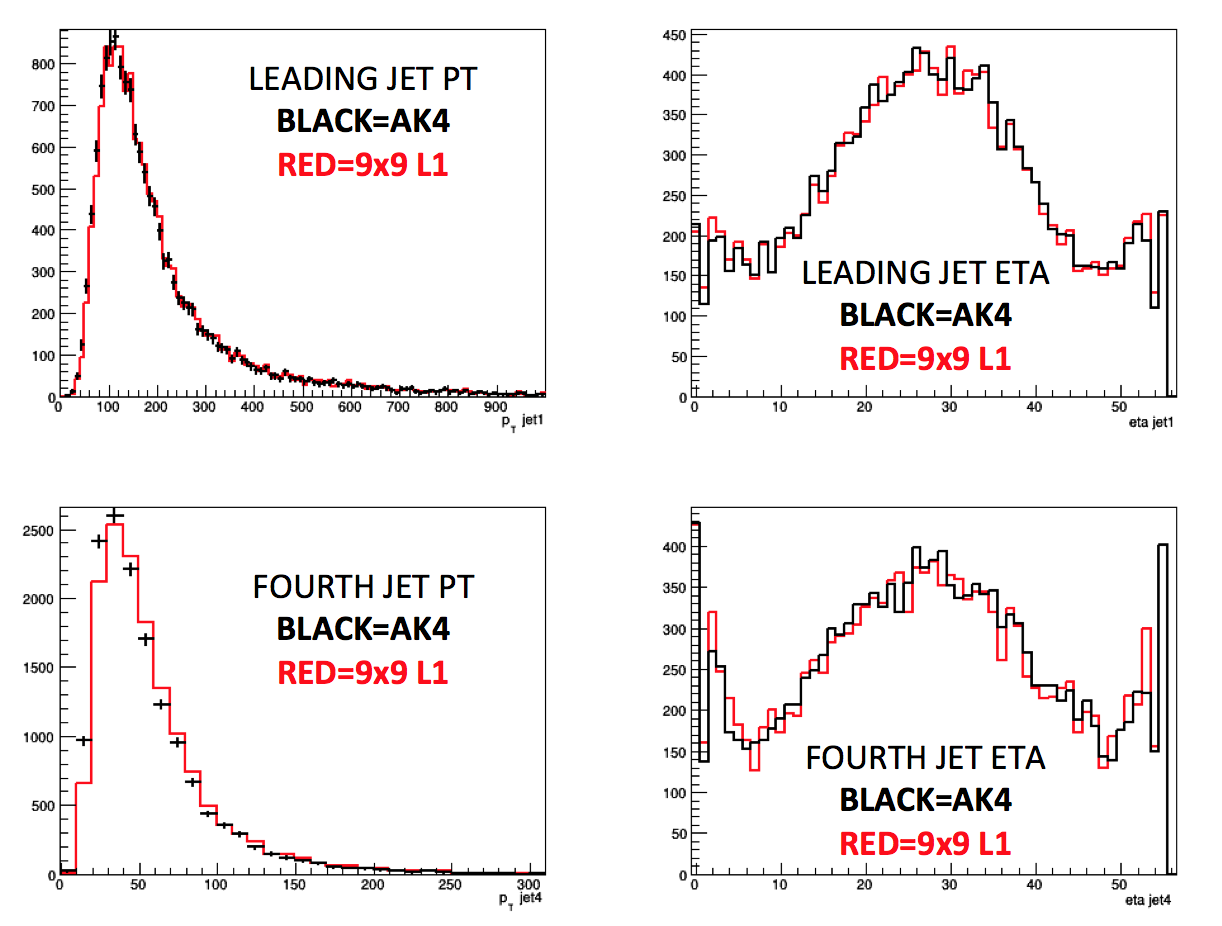
\includegraphics[width=1.0\linewidth]{figs/trigger/jet_l1s2_compak4}
	\end{center}
  \caption{A comparison between the upgrade Level-1 trigger (L1) jet
  algorithm and the anti-$k_T$ offline algorithm with R=0.4 
  (AK4), taking
  the Trigger Towers as input.  These plots are produced from a
  $t\bar{t}$ Monte Carlo simulation at $13$~TeV with pileup $\sim40$.
  The units for the pseudorapidity are in trigger tower units, which
  range from 0 at $\eta =-3$ to 56 at $\eta=3$.}
	\label{fig:ak4_comp}
\end{figure}

\subsection{Energy sums}

Along with finding jets in an event, the Level-1 trigger is required
to calculate energy sums, analogous to those discussed in
Sec.~\ref{sec:met_reco}.  These energy sums can take either the jets
or \TT as input. They currently include:
\begin{itemize}
\item{total $E_T$, the scalar sum of the transverse energy in all the \TT}
\item{\met, the inverse vector sum of the transverse energy in all the
\TT}
\item{\HT, the scalar sum of all Level-1 jets}
\item{\MHT, the inverse vector sum of all the Level-1 jets}
\end{itemize}

\section{Pileup subtraction}
\label{sec:pus}

\subsection{Characterising pileup}

On average, the decays from \PU are expected to be isotropically
distributed around the detector. However, there will be significant
event-by-event differences due to poisson fluctuations in the number
of \PU collisions. While the number of simultaneous interactions is
such that these fluctuations are significant it is advantageous to
correct for the \PU on a per-event basis. To be able to remove the
effects of \PU in the Level-1 trigger there needs to be a way remove
the objects that originate from \PU particles. Additionally, an
estimate of the average energy deposited in each event should be used
to correct the $E_T$ of the remaining objects. These procedures are
known collectively as \emph{\PUS}.

It is observed that the density of decays from \PU to
depend on their position in $\eta$ \cite{Cacciari2011}. This is
most likely caused by the differing response of the detector along its
length. The fact that the trigger only has access to
coarse calorimeter information with no tracks means these detector
effects are likely to be enhanced. It is therefore desirable for \PUS
algorithms to measure the \PU energy density near to the objects that
are corrected. This \emph{local} \PUS then requires a trade off
between the proximity to the object and the effects of
larger statistical fluctuations present when sampling a smaller area. 

A \emph{global} subtraction can be used to determine the average
energy density across the whole detector. This method is much less
susceptible to fluctuations and contamination from particles from the
hard-interaction, but does not take account of local fluctuations or
detector effects.

The ideal form of \PUS will remove the dependence of the Level-1
trigger rate and efficiency on the number of simultaneous interactions
in an event. It should do this in a way that improves the resolution
of object energy measurements in a way that increases the acceptance
of interesting physics events while allowing for the rejection of soft
QCD multijet processes. It is also important to take account of the
Level-1 trigger architecture when designing the algorithm to ensure
that it can be performed with a fixed latency. Different forms of \PUS
in the Level-1 trigger are outlined in this section and their
performance subject to this criteria is is examined in
Sec.~\ref{sec:jet_algo_performance}. 

\subsection{Global pileup subtraction}

A prominent method of \PUS is $\rho$-area correction
\cite{Cacciari:2007fd,Cacciari:2008gn}. It works by finding the
average energy per unit area in the calorimeter due to PU, $\rho$, and
subtracting it from each reconstructed jet. A favoured estimator for this
quantity is:
\begin{equation}
\rho\equiv median(\frac{p_{Tj}}{A_j}),
\end{equation}
where $p_{Tj}$ is the transverse momentum of a jet $j$, $A_j$ is its
area and the median is taken over all reconstructed jets in an event.
In this Chapter this form of \PUS is known as \emph{global $\rho$}. It
acts to remove half the jets in an event, the low energy half, and
correct down the energy of the remaining half. This works works
particularly well in high \PU cases as $\rho$ is insensitive to
fluctuations in the energy of interesting physics events. It is
possible to take account of $\eta$ dependence through a new variable
\emph{local $\rho$}, where the different values are calculated in
different $\eta$ ranges of the detector. This method loses robustness
as the number of jets that are sampled is lowered for each $\rho$
calculation.

The mean value of \rho, as a function of the number of interactions, is
shown in Fig.~\ref{fig:rho}. This is taken from a minimum bias \MC
simulation in which there is no visible hard interaction but only
overlaid \PU collisions. There is a good correlation between the
number of simultaneous collisions and \rho that passes through the
origin, indicating that it is indeed a reasonable measure of the \PU
in the event. 

\begin{figure}
	\begin{center}
		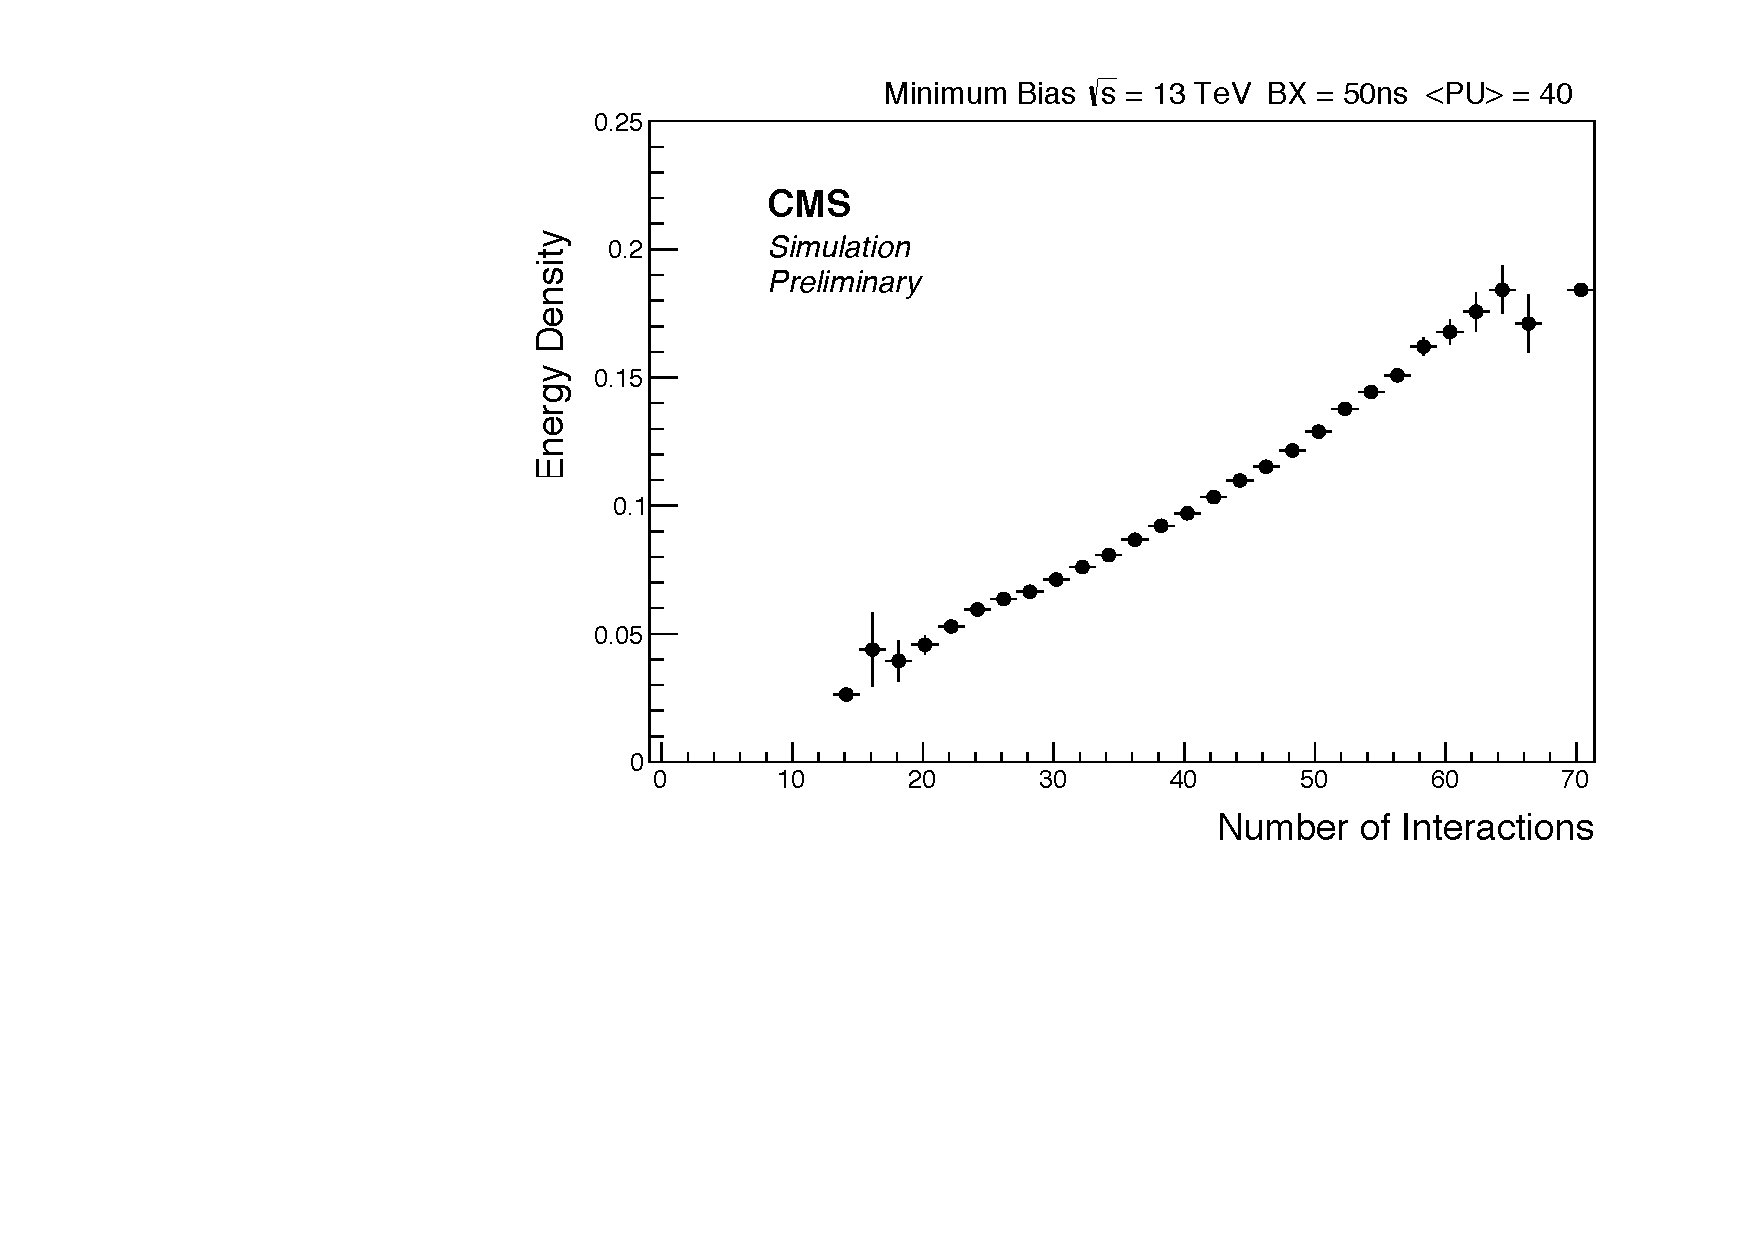
\includegraphics[width=0.8\linewidth]{figs/trigger/median}
  \caption{The median energy density, \rho, of Level-1 jets in the \CMS
  calorimeters as a function of the number of simultaneous collisions.
  This is taken from minimum bias \MC simulation at 13~\tev with a
  50~ns bunch crossing time}
	\end{center}
	\label{fig:rho}
\end{figure}

Global $\rho$ subtraction has a latency penalty in hardware as
the jets must be found before it can be calculated and subtracted from
their energies. Depending on the final firmware designs this can
present a problem and makes global \rho subtraction harder to perform
in hardware. Despite this fact, as global \rho is a popular and well
understood form of offline \PUS it acts as a good benchmark against
which to test other algorithms.

\subsection{Donut Subtraction}

As jets from the hard scatter are typically boosted objects, most of
their energy is deposited very close to the central \TT of the jet
algorithm \cite{JetProfile_pileup}. A typical energy profile of a jet
is shown in Fig.~\ref{fig:jetprofile}. In the case of isolated jets,
the ring $5$ \TT from the centre of the jet can be assumed to contain
only \PU.  The \emph{donut subtraction} algorithm therefore take the
energy per unit area in the ring of \TT surrounding the jet (shown in
Fig.~\ref{fig:donutstrips}) and scales
it up by the area of the jet. The resulting energy is then subtracted
from the jet to correct any \PU contamination. This kind of \PUS has
been applied in the analysis of heavy ion collisions at the \LHC
\cite{Cacciari:2010te}.

\begin{figure}
	\begin{center}
		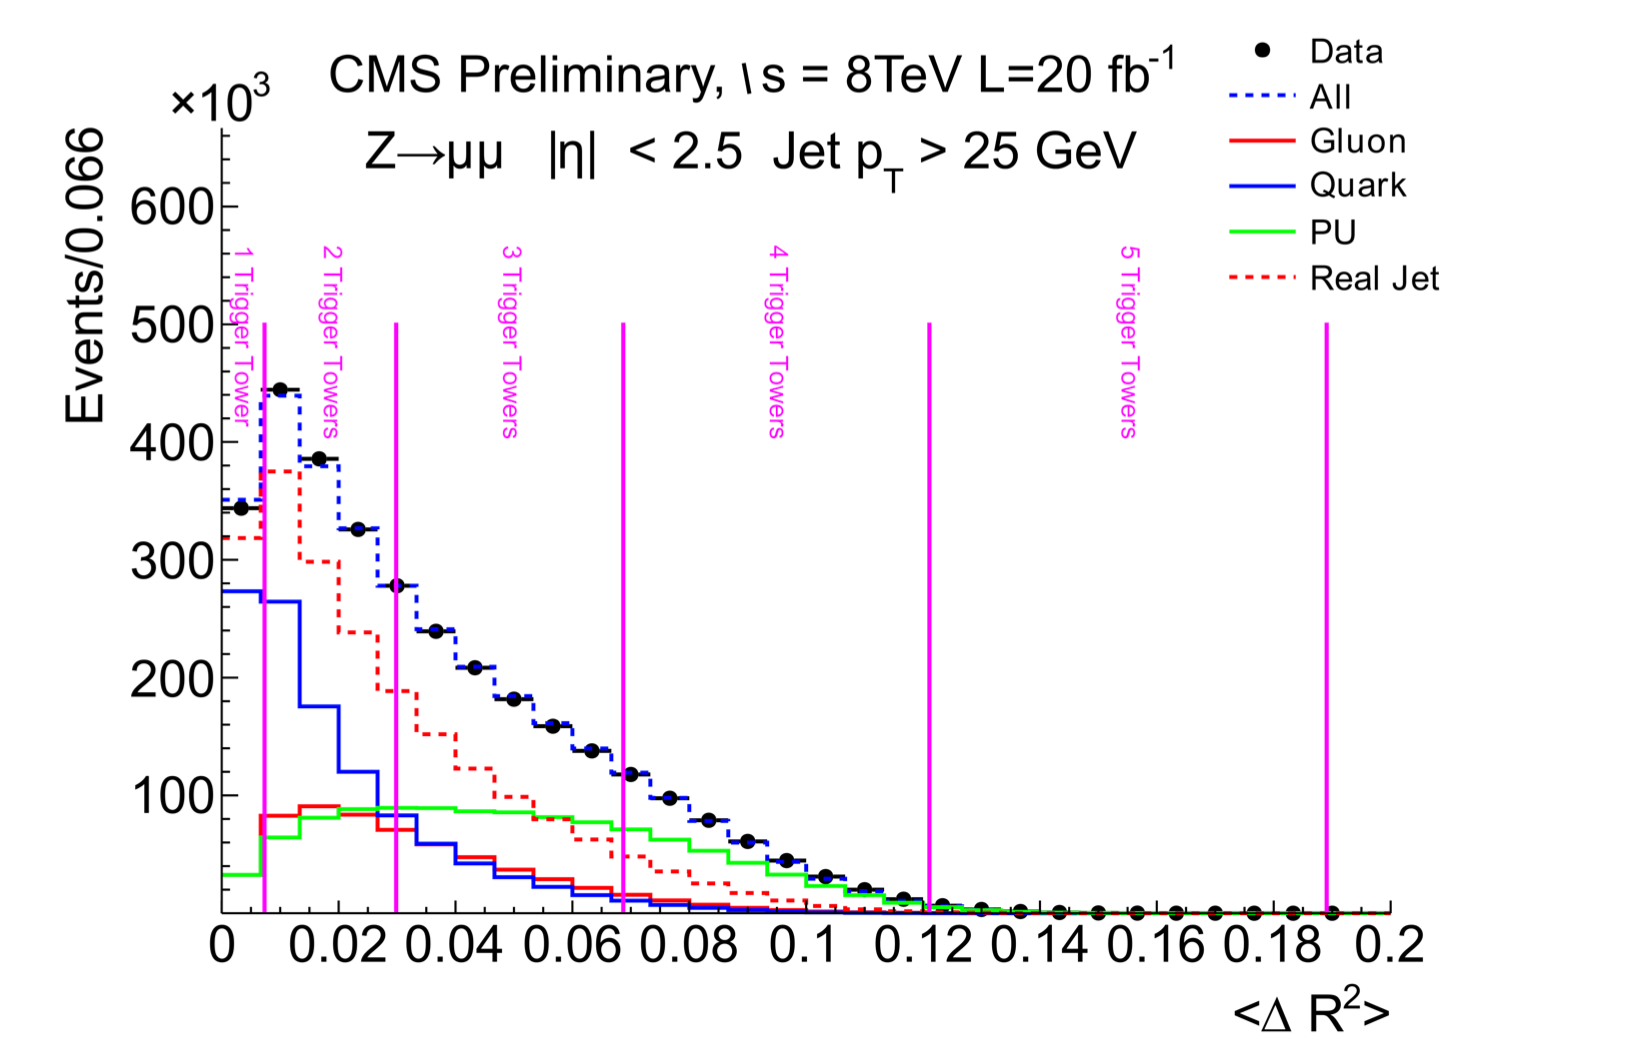
\includegraphics[width=0.8\linewidth]{figs/trigger/jetProfile}
  \caption{ Jet energy profile as a function of distance from the
  centre of the jet, $R$. The number of trigger towers that the
  distances corresponds to are shown in pink. Calculated for jets from
  a simulation of Z to $\mu\mu$ events \cite{JetProfile_pileup}}
	\end{center}
	\label{fig:jetprofile}
\end{figure}

This approach only works for correcting isolated jets, if one jet is
in the vicinity of another the energy in the donut can be increased to
above that of \PU. To mitigate this, only the median two $4\times1$
\TT strips of the four that make up the donut are used to calculate
the PU energy density. This reduces the chance that energy from
another jet will be counted as \PU and also removes strips that have
very little energy in them from a downward fluctuation in \PU
contamination. An example of the two strips that could be selected can
be seen in Fig.~\ref{fig:medianstrips}.

\begin{figure}[!t]
  \centering
  \subfloat[Strips considered for donut subtraction.]{
    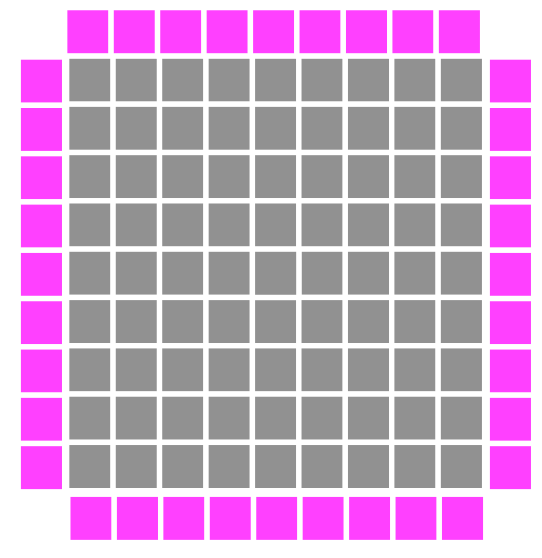
\includegraphics[width=0.3\textwidth]{figs/trigger/donut}
    \label{fig:donutstrips}
  }~ 
  \subfloat[Example of median energy strips.]{
    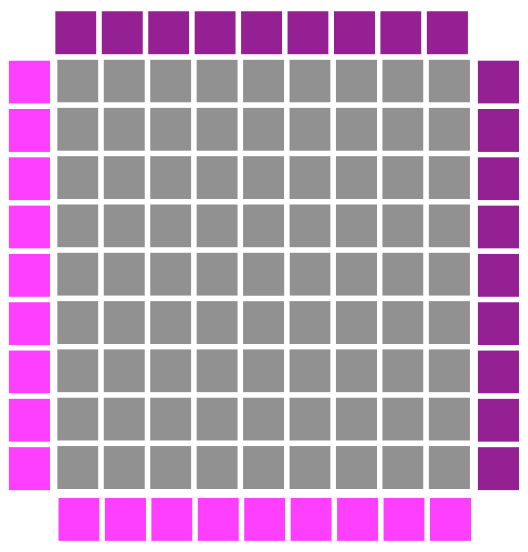
\includegraphics[width=0.3\textwidth]{figs/trigger/donut2}
    \label{fig:medianstrips}
  }~
  \subfloat[Strips considered for chunky donut subtraction.]{
    
\includegraphics[width=0.3\textwidth]{figs/trigger/chunkyDonut}
    \label{fig:chunkystrips}
  }\\
  \caption{Various configurations of \TT strips around the Level-1 jet
  algorithm window used for donut subtraction}
  \label{fig:alldonutstrips}
\end{figure}

One of the main issues with the donut subtraction algorithm is its
sensitivity to fluctuations. Contamination from other jets from the
hard scatter cause too much energy to be subtracted and in the case
that there are no \PU particles in the donut too little energy is
subtracted. This is mitigated by taking the median energy two strips
but can be further reduced by increasing the area covered by the
strips. The rings of \TT can be extended to be three towers wide,
known as a \emph{chunky} donut and illustrated in
Fig.~\ref{fig:chunkystrips}. This is particularly effective in
reducing the fluctuations in the positions of \PU particles with
respect to the jet in consideration.

To confirm that the energy in the median two strips of the  chunky
donut is a good measure of the \PU in the event, it is plotted against
the number of interactions for a minimum bias \MC sample in
Fig.~\ref{fig:donut_nint}. There is a good correlation that appears to
pass through the origin, implying it is indeed a good measure of \PU. 
% note that the fact that it passes through the origin for ttbar
% indicates that the median strips reduce hard scatter contamination

\begin{figure}
	\begin{center}
		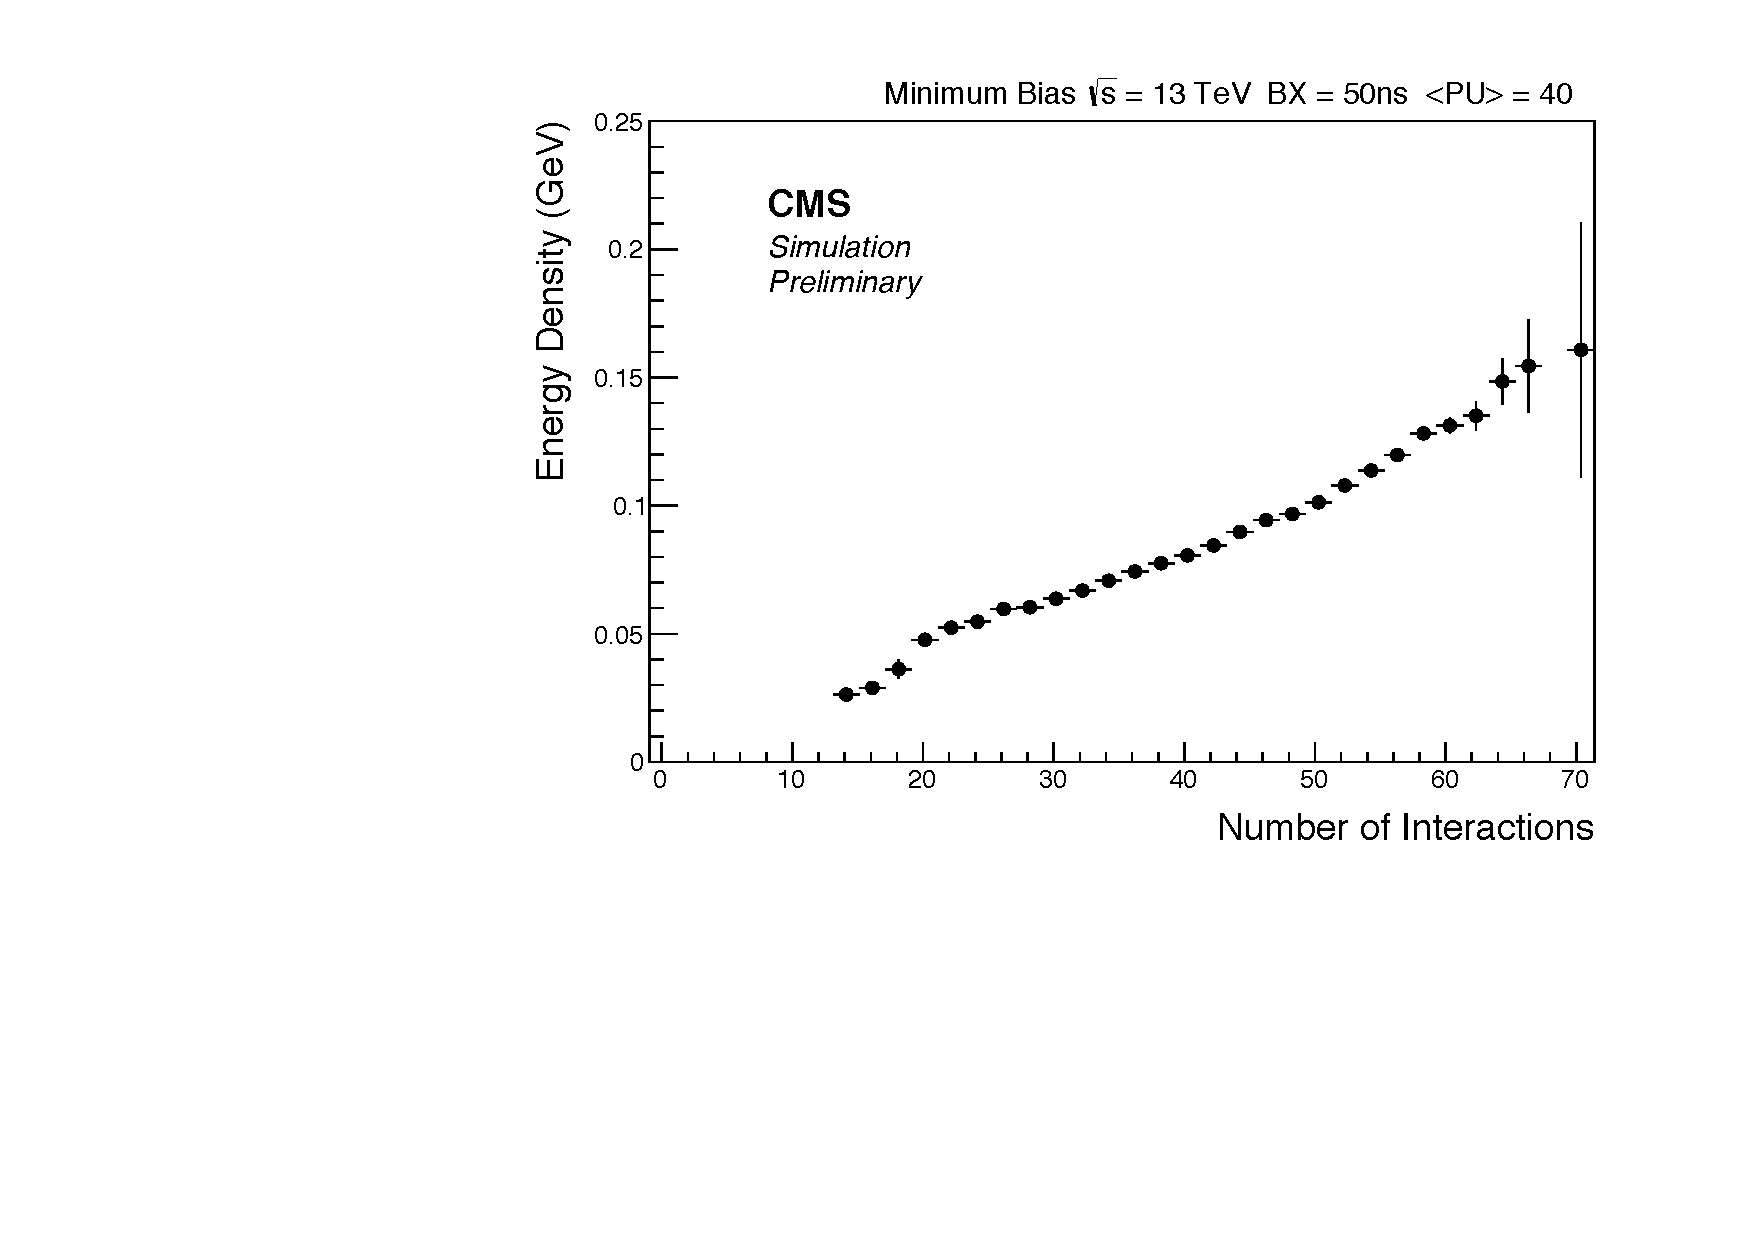
\includegraphics[width=0.8\linewidth]{figs/trigger/threestrips}
  \caption{The energy density in the median two $3\times 1$ \TT strips
  of a chunky donut around Level-1 jets in the \CMS calorimeters as a
  function of the number of simultaneous collisions. This is taken
  from minimum bias \MC simulation at 13~\tev with a 50~ns bunch
  crossing time}
	\end{center}
	\label{fig:donut_nint}
\end{figure}

In the implementation of the Level-1 jet finding algorithm in the
upgrade hardware , the \TT that make up the donut are already
available in memory. This means donut subtraction has a very low
latency penalty. This presents a significant advantage over a global
\PUS. 

\subsection{Jet seed threshold and zero suppression}

Donut subtraction helps to remove the effects of \PU on the
reconstructed high energy jets, but is less successful at removing the
soft jets that are purely from \PU interactions. A simple way of
reducing the number of soft jets is by introducing an energy threshold
on the \TT that can form a jet. The \TT that is considered for a jet
candidate in the algorithm outlined in
Section~\ref{sec:stage2_jetalgo} is required to be above a certain
energy, known as the seed threshold. This is very easy to implement in
hardware, and has the potential to save latency as it reduces the
number of jets that need to be made. A disadvantage is that it can
kill soft jets that originate from a primary vertex. It also does not
account for any $\eta$ dependence. For the studies in
Sec.~\ref{sec:jet_algo_performance} studies a seed of $2.5$~GeV was
chosen as a benchmark that appeared to kill PU jets without removing
jets above 10~GeV from a zero PU $t\bar{t}$ test sample. This is
demonstrated in Fig.~\ref{fig:noPUSeedTTbar}. As the Level-1 hardware
measures energy in units corresponding to 0.5~\gev (\emph{L1-units},
this is denoted as \emph{Seed 5}. 

\begin{figure}
	\begin{center}
		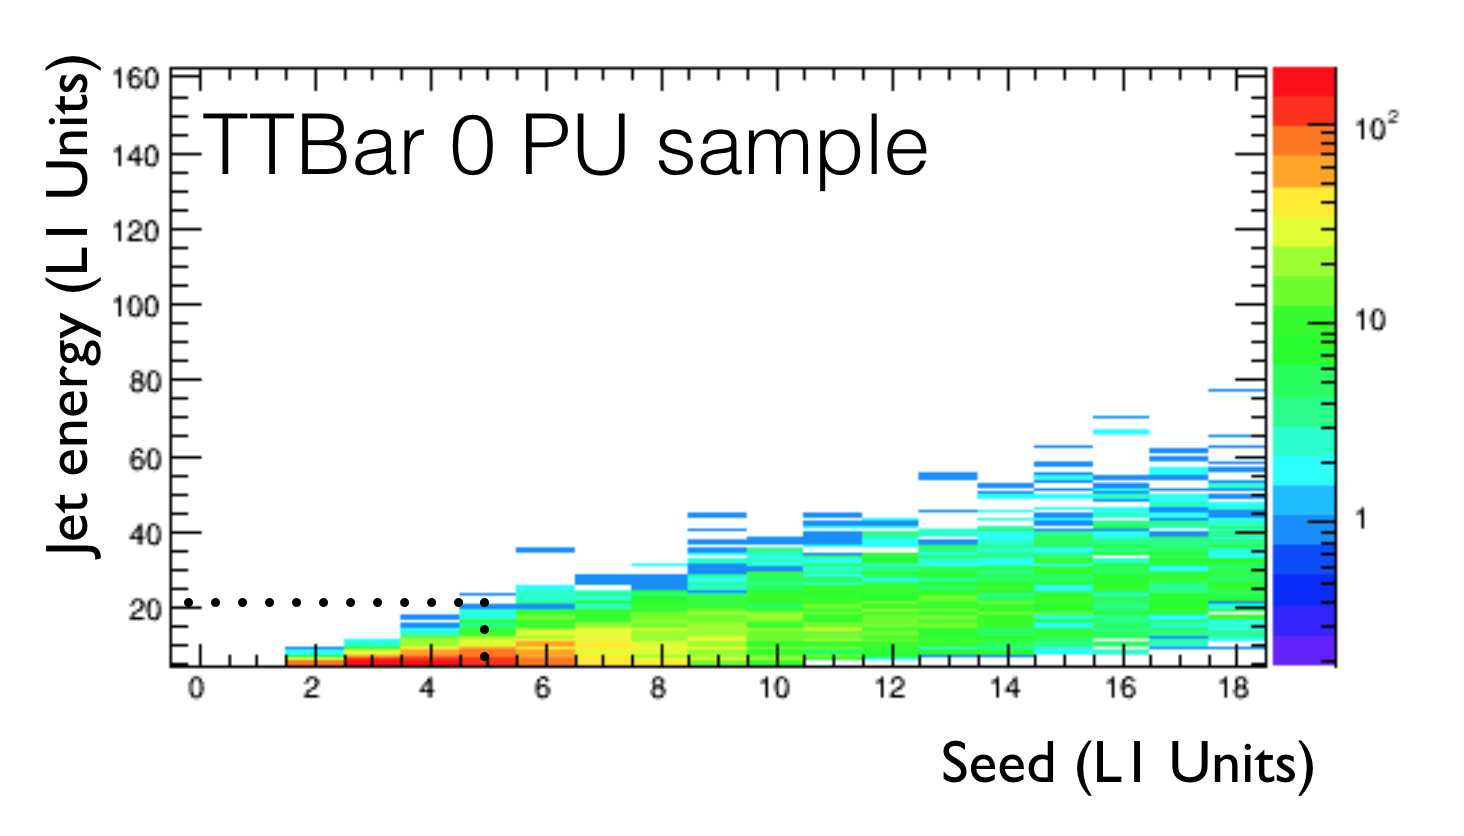
\includegraphics[width=0.8\linewidth]{figs/trigger/noPUSeedTTbar}
  \caption{The Level-1 jet energy vs seed threshold for a simulated
  sample of top quark pair production events with no overlaid \PU. The
  units of energy are \emph{L1-units}, which correspond to 0.5~\gev
  each. A seed threshold of 2.5~\gev only removes up to 10~\gev jets
  from the hard scatter.}
	\end{center}
	\label{fig:noPUSeedTTbar}
\end{figure}

To remove the effects of noise on the Level-1 trigger inputs, a
\emph{zero-suppression} is performed that requires \TT to have an
energy above 0.5~\gev before they are considered to have energy in at
all. As \PU is expected to result in much smaller energy deposits than
interesting physics processes, the effect of increasing the energy
that is suppressed to zero when building the jets also acts as a form
of \PUS. This form of \PUS is studied in
Sec.~\ref{sec:jet_algo_performance} and is named Tower Suppression
(TSup). Despite being very easy to implement in hardware this
algorithm does not adapt well to different \PU conditions and can
reduce the energy resolution of the jets.

\section{Level-1 jet energy calibration}
\label{sec:l1jec}

%mention something here about the PU140 calibration?

The inputs to the trigger do not exactly represent the offline quantities and the L1 jets have an more rigid size than the simulated Gen jets. By correcting the energy of the L1 jets through calibration it is possible to scale there energy to be closer to that of the Gen jets in an event \cite{l1jet-calibration}. It was necessary to produce a set of calibrations for L1 jets made with simulated data for the High Luminosity upgrade of the LHC, with PU of $\sim140$ per bunch crossing, for studies on the upgrade.
\\\\
To perform the calibration, L1 jets are matched to Gen jets produced from MC truth quantities (required to have $\Delta R<0.3$) for a collection of MC simulated events. For a particular bin of Gen $p_T$, a Gaussian is fit to the distribution of L1 jet $p_T$, giving a mean and its standard deviation. This value is plotted on the $x$ axis of the plot in Fig.~\ref{fig:calibfit}. The $y$ value is found by fitting in the same bin the ratio of the Gen and L1 $p_T$. The result is a set of points that can be fit with an appropriate function. To calibrate L1 jets in the future, the correction factor can be calculated by reading off the value of the fit function at a certain L1 $p_T$. 
\\\\
The performance of this calibration can be seen in Fig.~\ref{fig:calibclosure}. In this case the calibration is effective down to around $30$~GeV. This is expected as the fit was only valid until this value. In high PU samples the low energy L1 jets are heavily contaminated. This results in the Gen jets not being matched to the correct corresponding L1 jet, characterised by the turn over in the ratio as the $p_T$ decreases.
%why calibrate
%calibration theory- fit
% \begin{figure}
% 	\begin{center}
% 		\includegraphics[width=0.6\linewidth]{pu140_calibrationfit}
% 	\end{center}
% 	\caption{A fit to the L1 $p_T$ against its ratio with Gen for a particular $\eta$ bin. This fit is used to calculate calibration factors for the L1 jets.}
% 	\label{fig:calibfit}
% \end{figure}
% %explain turnover
% %closure test- plots
% \begin{figure}
% 	\begin{center}
% 		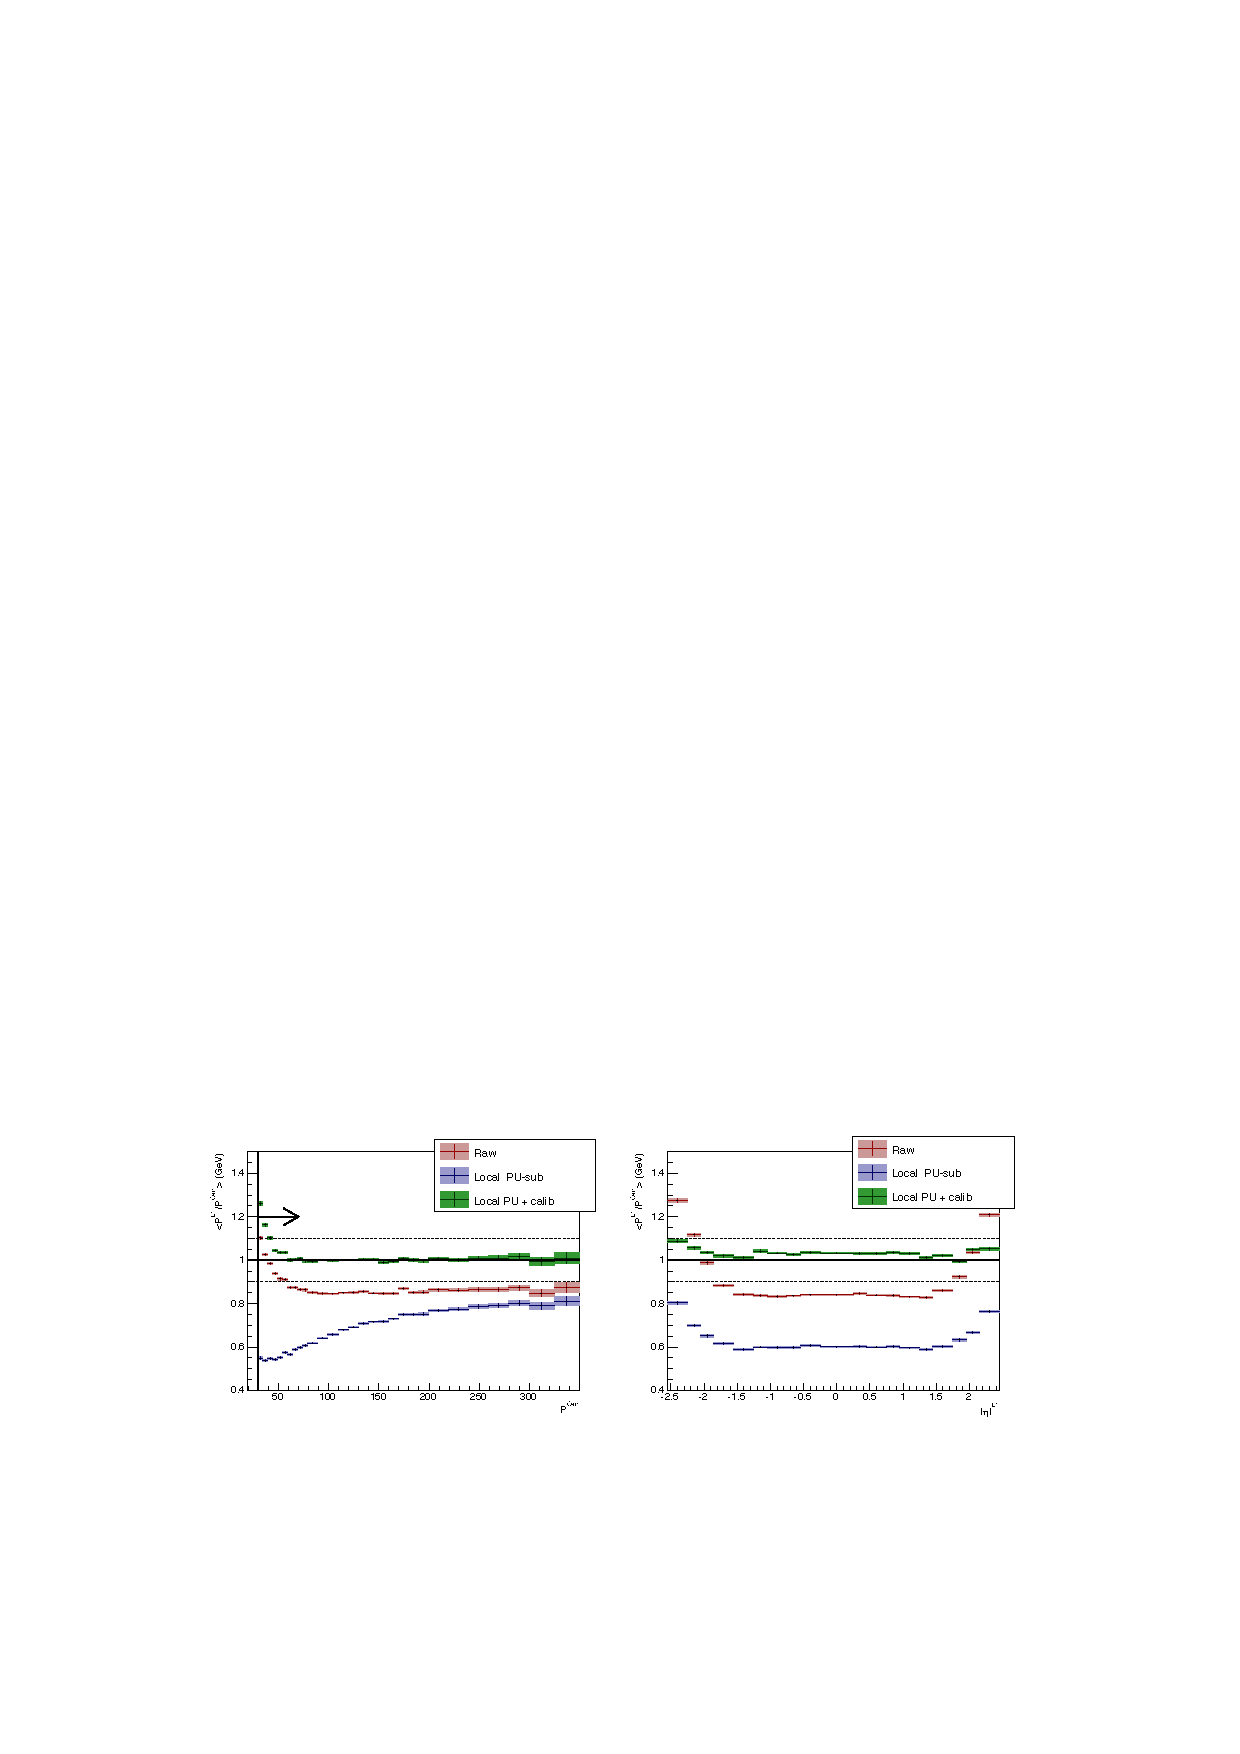
\includegraphics[width=1.0\linewidth]{pu140_calib_closure}
% 	\end{center}
% 	\caption{The ratio of L1 jets with Gen before and after they are calibrated, demonstrating the effectiveness of the calibration \cite{nick-pu140calib}}
% 	\label{fig:calibclosure}
% \end{figure}

\section{Performance of the upgraded algorithm}

\label{sec:jet_algo_performance}
The performance of the jet algorithm with the above methods of PUS was tested on 13~TeV MC simulation. A comparison is made to the jets produced by the GCT as it was in 2012. To investigate rates a zero bias neutrino gun sample was used. To test physics performance and compare to AK4 generator level jets (Gen) a $t\bar{t}$ signal sample was used . L1 jets are calibrated with the method as outlined in Section~\ref{sec:pu140_calib}.
%\footnote{/Neutrino\_Pt-2to20\_gun/Fall13dr-tsg\_PU40bx50\_POSTLS162\_V2-v1/GEN-SIM-RAW}
%\footnote{/TT\_Tune4C\_13TeV-pythia8-tauola/Fall13dr-tsg\_PU40bx50\_POSTLS162\_V2-v1/GEN-SIM-RAW}
\\\\
Fig.~\ref{fig:matchingeff} shows the efficiency of Gen jets being reproduced at L1 as a function of their $p_T$. If a Gen jet has a corresponding L1 jet within a radius $R=0.5$ it is counted as matched. This radius is chosen as the distance from the centre of a L1 jet to the corner of its $9\times9$ square. With the proposed Stage 2 jet algorithm, there is close to $100\%$ efficiency above $70$~GeV. The seed appears to be quite aggressive for low $p_T$ jets, but the donut subtraction does not remove any signal jets. The improved granularity greatly improves the performance over the GCT.
%Checked matching to gen, dr 32, inefficiencies caused by algorithm - gct bad
% \begin{figure}
% 	\begin{center}
% 		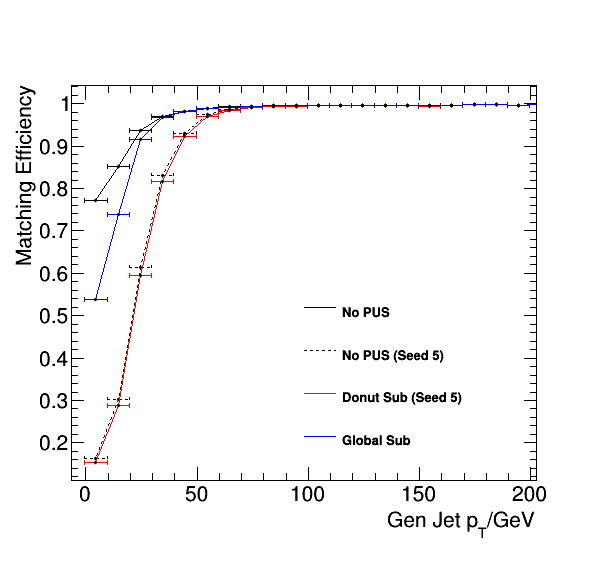
\includegraphics[width=0.6\linewidth]{performance/matchingeff_alljet}
% 	\end{center}
% 	\caption{The efficiency with which a Gen jet has a corresponding L1 jet within a radius, $R=0.5$. This is carried out for all Gen jets in 70~000 $t\bar{t}$ events.}
% 	\label{fig:matchingeff}
% \end{figure}
\\\\
\noindent To characterise the energy performance of the L1 jets, turnon curves are plotted in Fig.~\ref{fig:turnons}. These are made by matching the Gen jets to L1 jets, requiring $\Delta R<0.5$ and taking the matched Gen $p_T$ distribution without a cut on L1 jets and one with a cut on the L1 jets, then dividing the two histograms. The fourth leading jet of a $t\bar{t}$ sample is used as it displays the biggest discrepancy between algorithms. By $80$~GeV the PUS doesn't affect the resolution except for donut subtraction which appears to be over subtracting energy in a small number of cases.
% \begin{figure}
% 	\begin{center}
% 		\includegraphics[width=0.5\linewidth]{performance/turnon_jet4_40}\put(-42,203){(a)}
% 		\includegraphics[width=0.5\linewidth]{performance/turnon_jet4_80}\put(-42,203){(b)}
% 	\end{center}
% 	\caption{The proportion of remaining Gen jets matched to fourth leading L1 jets after performing a cut on L1 of (a) 40GeV, (b) 80GeV.}
% 	\label{fig:turnons}
% \end{figure}
%turnons - how energy matched to gen - gct bad
\\\\
\noindent To measure the performance of the PUS algorithms removing soft QCD PU jets, the rate against the number of interactions is plotted for the zero bias sample for a representative $p_T$ cut of $30$~GeV, Fig.~\ref{fig:ratenvtx}. The PUS clearly lowers the dependence on the number of interactions and reduces the rate of jets passing the cut, it is performing as it should. It seems that the seed threshold is the most effective at killing soft QCD, with donut subtraction on top not making much difference. GCT jets are incredibly sensitive to PU, further motivating the trigger upgrade.
% \begin{figure}
% 	\begin{center}
% 		\includegraphics[width=0.5\linewidth]{performance/ratenvtx_neutrino_jet1}\put(-42,203){(a)}
% 		\includegraphics[width=0.5\linewidth]{performance/ratenvtx_neutrino_jet4}\put(-42,203){(b)}
% 	\end{center}
% 	\caption{The relative rate of L1 jets with $p_T>30$~GeV after PUS for the leading jet, (a), and fourth leading jet, (b), for $70 000$ zero bias events as a function of the number of interactions (NVTX)}
% 	\label{fig:ratenvtx}
% \end{figure}
%level of soft qcd pileup subtraction- rate vs nvtx
\\\\
\noindent To ensure that the PUS algorithms are not too aggressive, efficiency is plotted against the rate from a zero bias sample given a certain $p_T$ cut. Efficiency is defined as the fraction of events with a lead Gen jet of $p_T>50$~GeV that have a lead L1 jet that is matched to a Gen jet ($\Delta R<0.5$). Ideally the efficiency remains close to one while reducing as much rate as possible. It can be seen in Figure~\ref{fig:rateeff} that for the leading jet very good efficiency is retained in all cases, with the fluctuations in donut subtraction affecting it.
% \begin{figure}
% 	\begin{center}
% 		\includegraphics[width=0.6\linewidth]{performance/jet1RateEff}
% 	\end{center}
% 	\caption{The normalised rate against efficiency for various PUS schemes. Efficiency is defined as the fraction of events with a lead Gen jet of $p_T>50$~GeV that have a lead L1 jet that is matched to a Gen jet (dR<0.5). Based on a $t\bar{t}$ and zero bias sample.}
% 	\label{fig:rateeff}
% \end{figure}
%\begin{figure}
%	\begin{center}
%		\includegraphics[width=0.5\linewidth]{performance/rateseff_jet1}\put(-42,203){(a)}
%		\includegraphics[width=0.5\linewidth]{performance/rateseff_jet4}\put(-42,203){(b)}
% 	\end{center}
%	\caption{Given a particular $p_T$ cut on a level 1 jet the proportion of remaining leading, (a), and fourth %leading, (b), jets is plotted for a zero bias sample against a $t\bar{t}$ sample. The rate is represented by the %zero bias sample and the efficiency by the $t\bar{t}$}
%	\label{fig:rateeff}
%\end{figure}
%maintaining signal- rateseff
\\\\
\noindent The other purpose of PUS is to correct the energy of L1 jets contaminated with PU. The resolution of the jets as compared to Gen is defined as $\frac{p_T^{L1}-p_T^{Gen}}{p_T^{Gen}}$, being zero for perfect agreement. The PUS should act to remove the dependence of the resolution on the number of interactions in an event. In Figure~\ref{fig:resolution} it can be seen that the donut and global $\rho$ subtraction do flatten out the resolution for a representative bin of $p_T$ and $\eta$, whereas the seed on its own does not. 
% \begin{figure}
% 	\begin{center}
% 		\includegraphics[width=0.6\linewidth]{performance/pt_20to40_eta_-28to-14}
% 	\end{center}
% 	\caption{The resolution of L1 jets with $20<p_T<40$~GeV and with $-3<\eta<-1.2$ as a function of the number of interactions (NVTX)}
% 	\label{fig:resolution}
% \end{figure}
%correcting hard jets- response
\\\\
\noindent As a final performance test, the $H_T$ and $\cancel{H}_T$ as defined in Section~\ref{sec:alphaT} are plotted. If the PUS is too aggressive the $H_T$ will be too low when compared to Gen, or too high if it under subtracts. Figure~\ref{fig:htmht} shows that jets with a seed threshold most closely reproduce the $H_T$. Overall the PUS methods are under subtracting, however. The PUS does not improve the $\cancel{H}_T$ distribution, this is expected in the case that PU is distributed evenly.
% \begin{figure}
% 	\begin{center}
% 		\includegraphics[width=0.5\linewidth]{performance/ht_ttbar}\put(-42,203){(a)}
% 		\includegraphics[width=0.5\linewidth]{performance/mht_ttbar}\put(-42,203){(b)}
% 	\end{center}
% 	\caption{(a) The distribution of the total energy of jets in each event ($H_T$). (b) The distribution of the missing momentum of jets in an event ($\cancel{H}_T$).}
% 	\label{fig:htmht}
% \end{figure}
%not killing important jets- ht mht
\\\\
\noindent The proposed Stage 2 jet algorithm performs well with respect to the previous GCT algorithm. With the introduction of PUS, the more challenging conditions at 13TeV in Run 2 can start to be tamed. The rate of reconstructed jets can be reduced without sacrificing too much efficiency. Global subtraction and donut subtraction both help to remove the dependence of the energy of signal jets on PU. Due to fluctuations in the donut subtraction, the efficiency takes a hit, but it is better at reproducing the $H_T$ distribution than global $\rho$. This is just the beginning of the investigation of PUS for L1 jets, further investigation is required to optimise the parameters used and compare to other PUS schemes.

% \begin{figure}
%   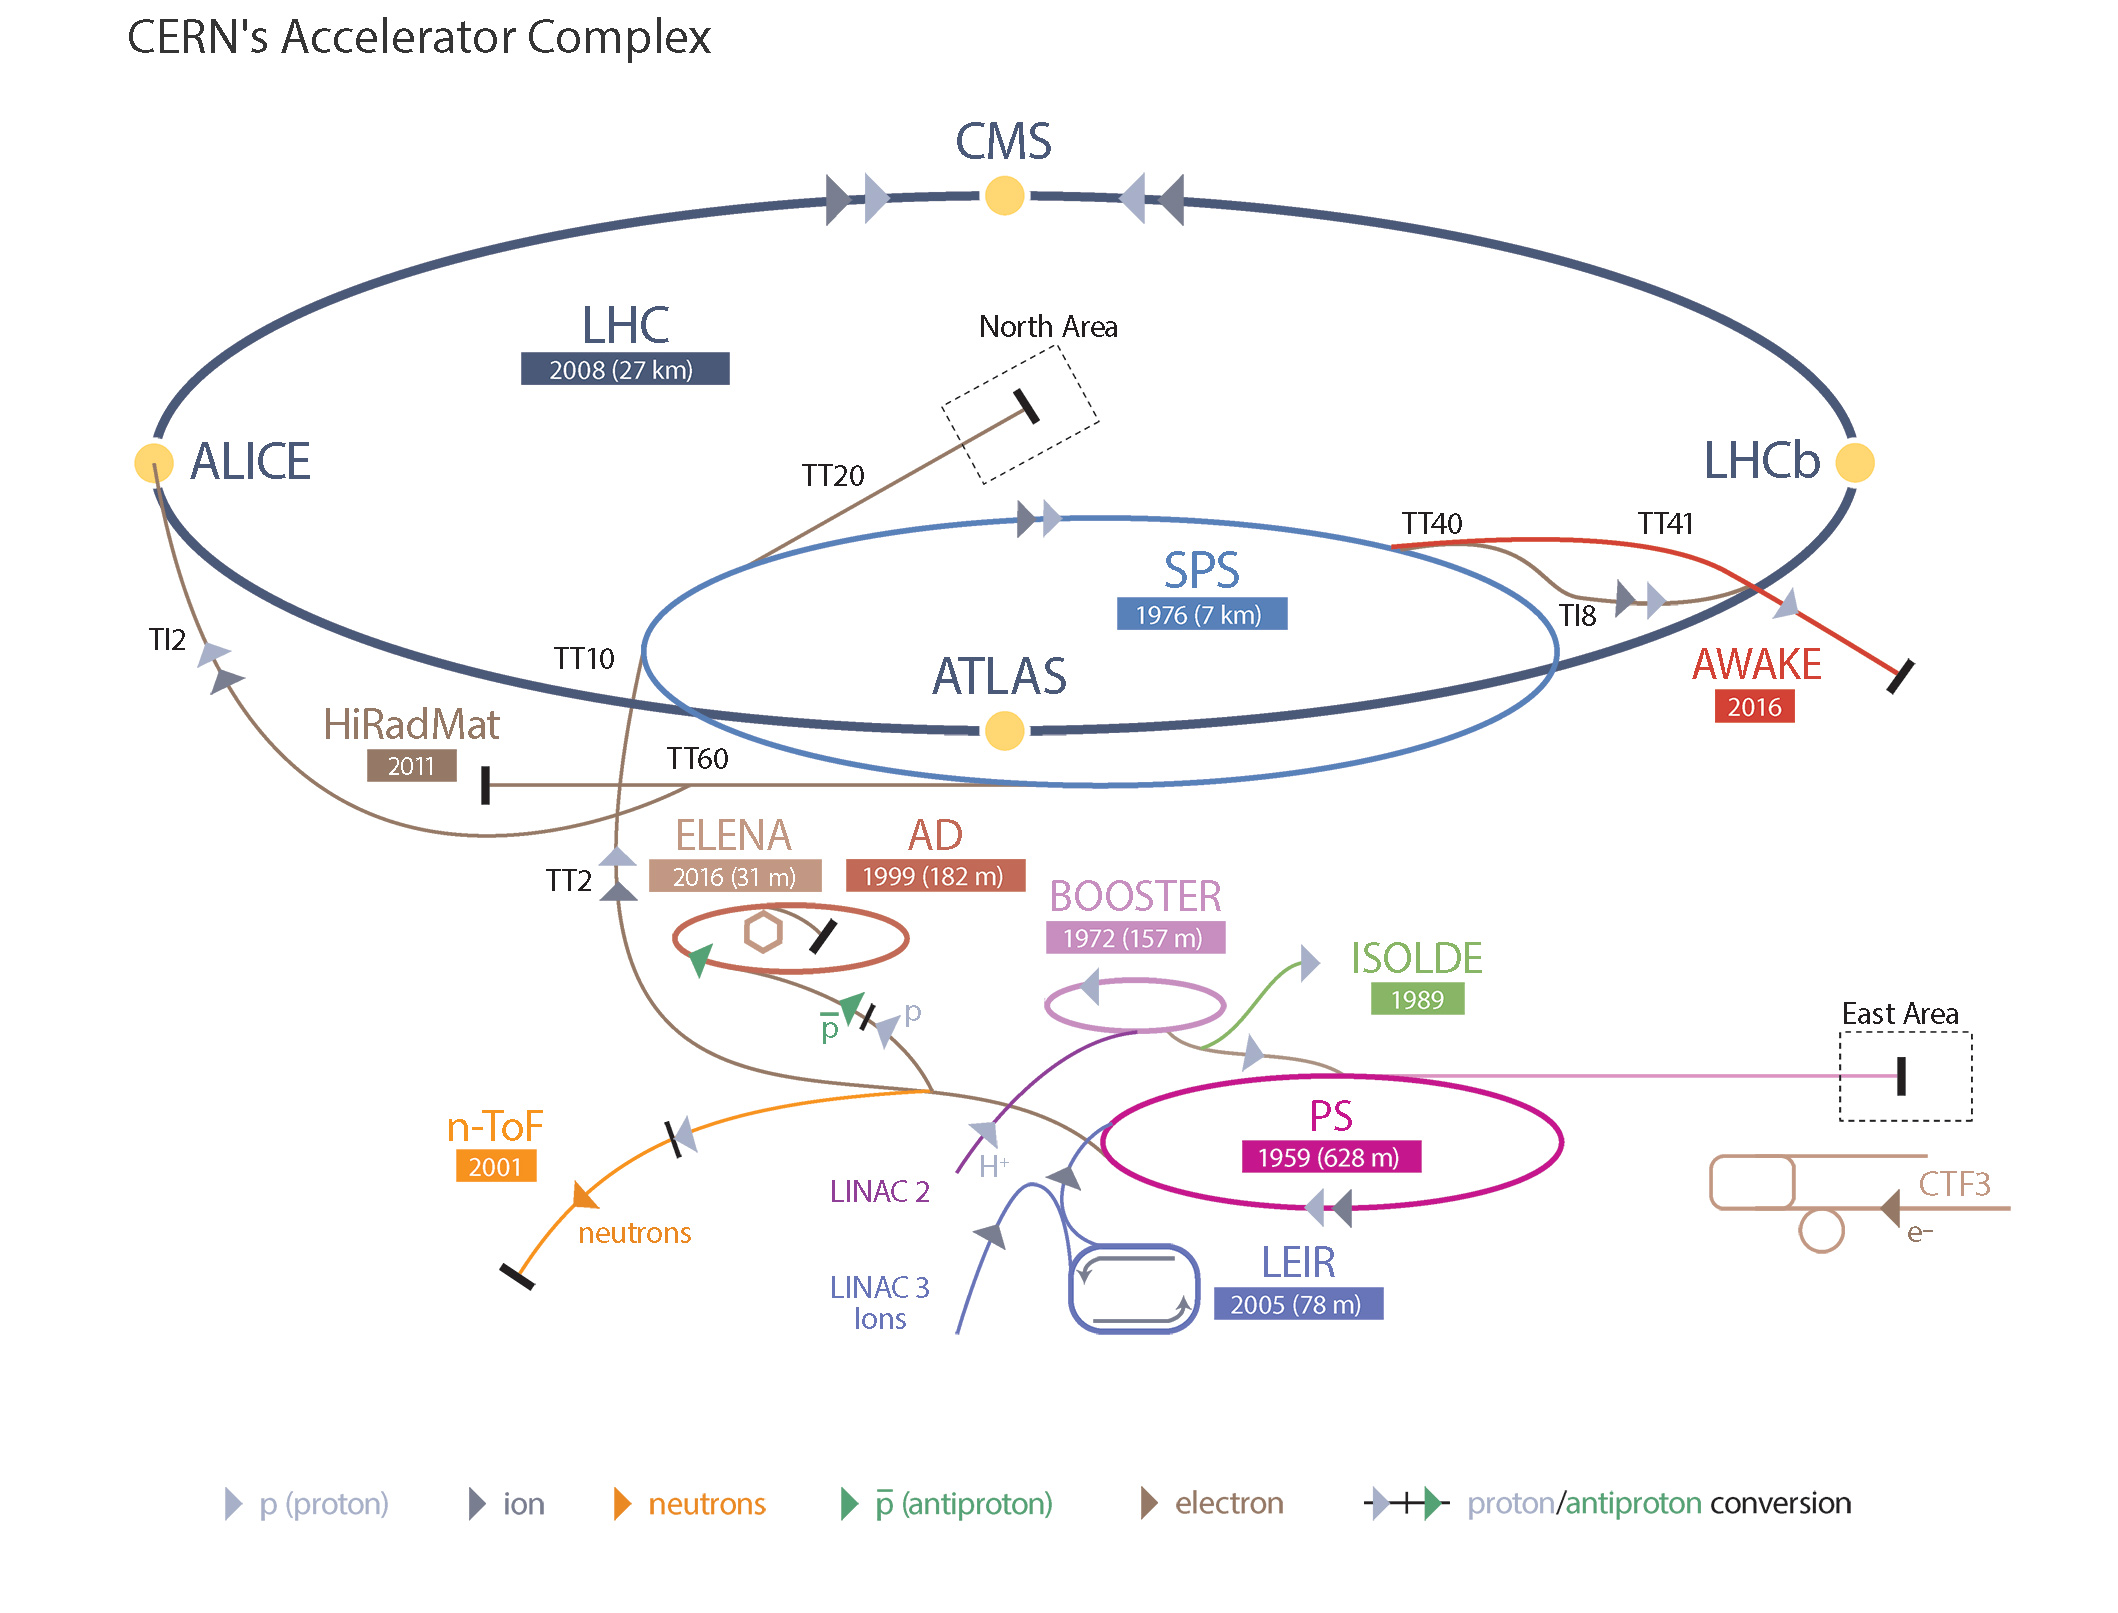
\includegraphics[width=\largefigwidth]{figs/LHC_default}
%   \caption[]%
%   {A representation of the CERN accelerator complex that
%   accelerates hadrons to high energies within the \LHC
%   \cite{stfc:lhc}}%
%   \label{fig:lhc}
% \end{figure}

\section{Emulator validation}
\label{sec:l1jec}

%put something here??

